\documentclass[12pt]{article}%
\usepackage{amsfonts}
\usepackage{fancyhdr}
\usepackage{comment}
\usepackage[a4paper, top=2.5cm, bottom=2.5cm, left=2.2cm, right=2.2cm]%
{geometry}
\usepackage{times}
\usepackage{amsmath}
\usepackage{listings}
\usepackage{changepage}
\usepackage{amssymb}
\usepackage{graphicx}%
\usepackage{amsmath} 
\setcounter{MaxMatrixCols}{30}
\newtheorem{theorem}{Theorem}
\newtheorem{acknowledgement}[theorem]{Acknowledgement}
\newtheorem{algorithm}[theorem]{Algorithm}
\newtheorem{axiom}{Axiom}
\newtheorem{case}[theorem]{Case}
\newtheorem{claim}[theorem]{Claim}
\newtheorem{conclusion}[theorem]{Conclusion}
\newtheorem{condition}[theorem]{Condition}
\newtheorem{conjecture}[theorem]{Conjecture}
\newtheorem{corollary}[theorem]{Corollary}
\newtheorem{criterion}[theorem]{Criterion}
\newtheorem{definition}[theorem]{Definition}
\newtheorem{example}[theorem]{Example}
\newtheorem{exercise}[theorem]{Exercise}
\newtheorem{lemma}[theorem]{Lemma}
\newtheorem{notation}[theorem]{Notation}
\newtheorem{problem}[theorem]{Problem}
\newtheorem{proposition}[theorem]{Proposition}
\newtheorem{remark}[theorem]{Remark}
\newtheorem{solution}[theorem]{Solution}
\newtheorem{summary}[theorem]{Summary}
\newenvironment{proof}[1][Proof]{\textbf{#1.} }{\ \rule{0.5em}{0.5em}}
\usepackage{color}

\definecolor{dkgreen}{rgb}{0,0.6,0}
\definecolor{gray}{rgb}{0.5,0.5,0.5}
\definecolor{mauve}{rgb}{0.58,0,0.82}

\lstset{frame=tb,
  language=MATLAB,
  aboveskip=3mm,
  belowskip=3mm,
  showstringspaces=false,
  columns=flexible,
  basicstyle={\small\ttfamily},
  numbers=none,
  numberstyle=\tiny\color{gray},
  keywordstyle=\color{blue},
  commentstyle=\color{dkgreen},
  stringstyle=\color{mauve},
  breaklines=true,
  breakatwhitespace=true,
  tabsize=3
}

\newcommand{\Q}{\mathbb{Q}}
\newcommand{\R}{\mathbb{R}}
\newcommand{\C}{\mathbb{C}}
\newcommand{\Z}{\mathbb{Z}}

\begin{document}

\title{Project 2}
\author{Shad Mahmod \\
Modelling Complex Systems}
\date{\today}
\maketitle
\section{Population dynamics}

-
 

\subsection{Basic population model}
\subsubsection{Initial model}
An initial simulation shows (see figure \ref{fig:5b}) differentiating behaviors for different values of b. In this simulation, the number of sites and the initial size of the population was set to 1000. \\� \\
\begin{figure}[htbp]
	\centering
	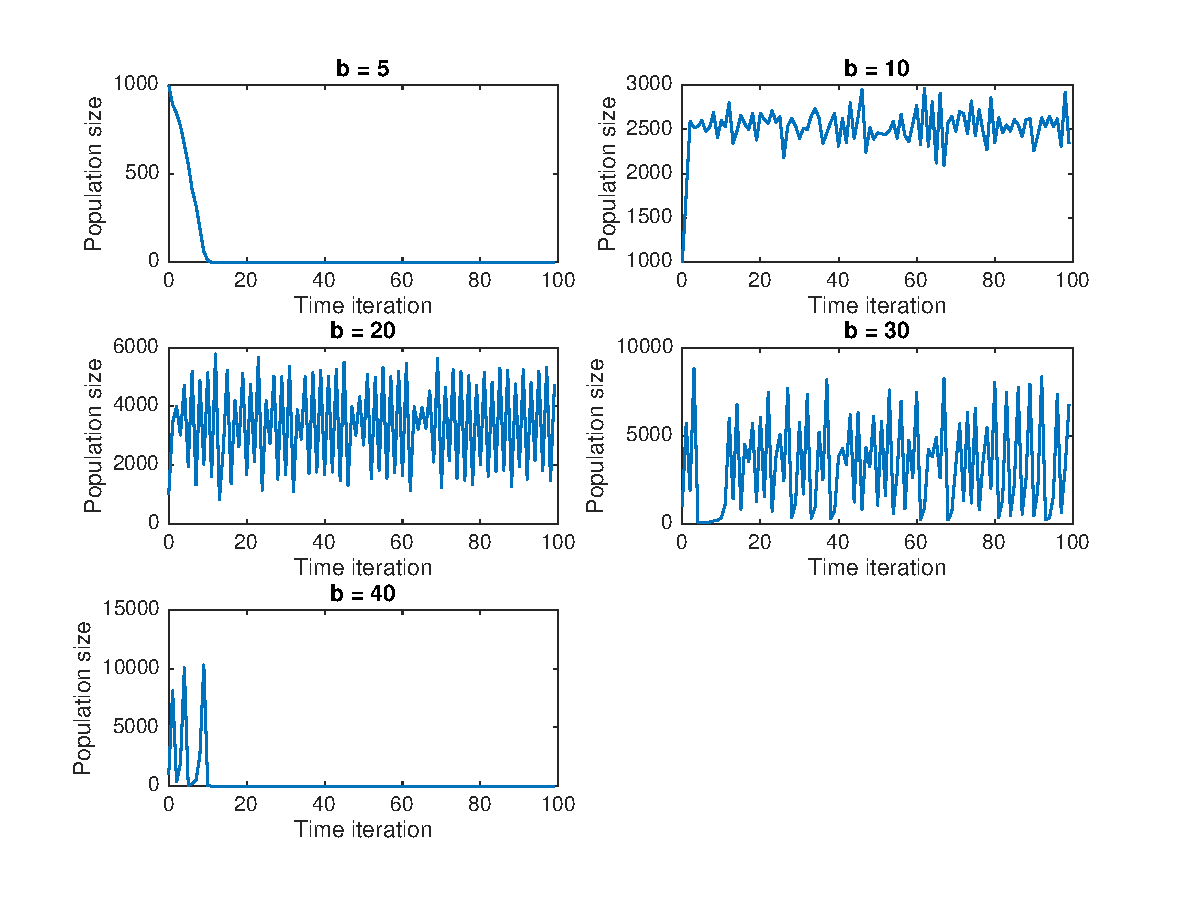
\includegraphics[scale=0.7]{figures/5bPop.eps}
	\caption{The number of people at different timesteps for different values of b. The initial size of the population was 1000 in all the cases as well as the number of sites.}
    \label{fig:5b}
\end{figure}
When b = 5 the population rapidly decreases towards 0.  The reason for this is that the offspring is not large enough to maintain a population. The number of sites that have a exactly a population of two at the inital timestep will probably by less than 200 (PROVE THIS!!!), so at the next timestep even fewer persons will be distributed amongst the sites and the overall trend will be negative. \\ \\
The case where b = 10 seems to be reaching a stable (in the sense that fluctuations from the mean are fairly small +-500) state after the first couple of iterations where it oscillates around 2500. Increasing b to 20 produces a somewhat similar behavior (oscillation around a constant value) with the difference that the the peak to peak values seem to be 3-4 times higher. So instead of diverging with +-500 it diverges with about +-1750.\\ \\
When b = 30 we note that the peak to peak values can be even larger, at one instance it goes from around 8000 to 1, a decline that is expected due to the smal number of sites, however it quickly bootstraps its way back to a higher number afterwards. It the continues to oscillate. \\ \\
Finally, in the case of b = 40, we see that the simulation renders a couple of oscillations that are followed by the decimation of the whole population. Since the population now is 0 it is unable to reproduce and stays at this value. In the case of b = 40 the reason for the extinction is overpopulation. At the timestep before extinction, the population hits 10000 which happens to render a state in which there are no sites with population size 2.

\subsubsection{Changing the initial population size}
If the value of the initial population is decreased too much, another problem will arise. In this case the initial number of sites in which the population is two might be too small, in which case the population at the next timestep is even smaller and might which leads to an more deteriorating state. This is seen in figure \ref{fig:5b2} in which only the case of b = 50 manages to repopulate the system of sites to a "healthy" level.
\begin{figure}[htbp]
	\centering
	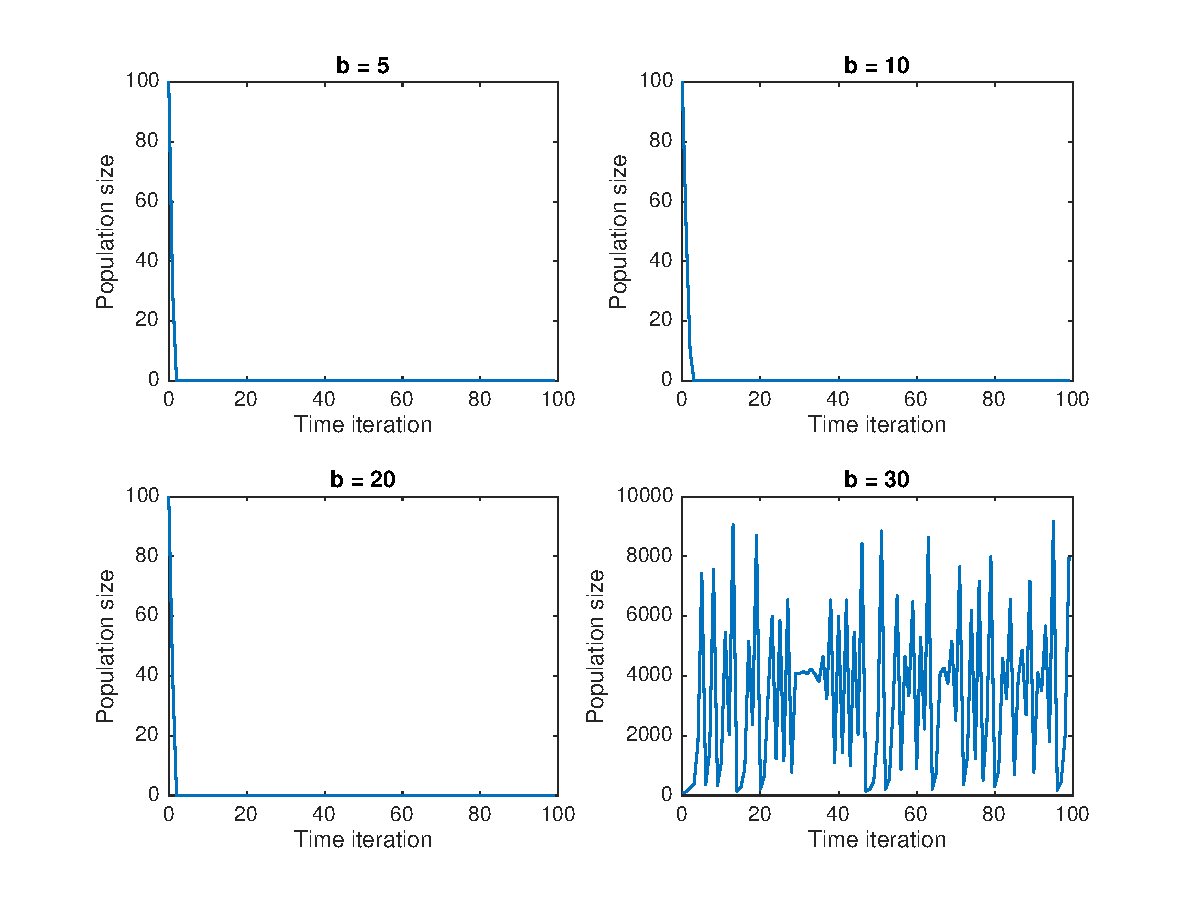
\includegraphics[scale=0.7]{figures/A_0small.eps}
	\caption{The number of people at different timesteps for different values of b. The initial size of the population was 100 in all the cases and the number of sites was 1000}
    \label{fig:5b2}
\end{figure}
If the initial number of sites with a population of two is high enough, then the system might be able to grow and sustain itself. In \ref{fig:5b2c} the system with b = 20 has managed to repopulate itself.
\begin{figure}[htbp]
	\centering
	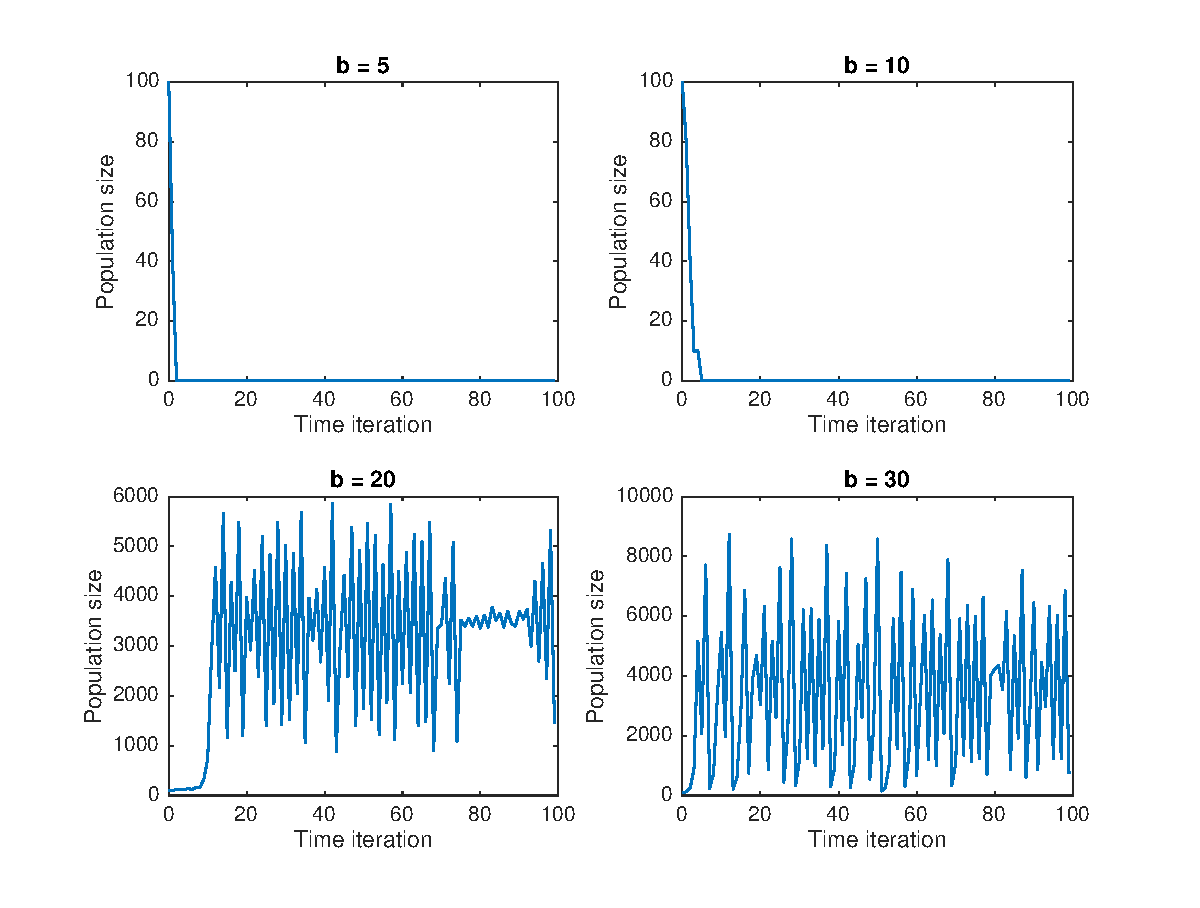
\includegraphics[scale=0.7]{figures/A_0small2.eps}
	\caption{The number of people at different timesteps for different values of b. The initial size of the population was 100 in all the cases and the number of sites was 1000}
    \label{fig:5b2c}
\end{figure}
\subsection{Mean-field equation}
In order to find the mean field approximation we must find the expected next state given the current state.
\begin{align*}
E(a_{t+1}| a_t) = h \sum_{k=0}^\infty P(\text{k at site i }| a_t)\phi(k)
\end{align*}
Where $\phi(k)=\left\{
  \begin{array}{@{}ll@{}}
    2 & \text{if}\ k = 2  \\
    0 & \text{otherwise}  \\
  \end{array}\right.$ is our interaction function. We assume that the number of people at sites is poisson distributed
  \begin{align*}
  P(\textit{k at site}�|�a_t) = \frac{(\frac{a_t}{n})^ke^\frac{-a_t}{n}}{k!}
  \end{align*}
We now make the assumption that $a_{t+1} = E(a_{t+1}|a_t)$
\begin{align*}
a_{t+1}  &= n \sum_{k=0}^\infty  \frac{(\frac{a_t}{n})^ke^\frac{-a_t}{n}}{k!} \phi(k) \\
& = n \frac{(\frac{a_t}{n})^2e^\frac{-a_t}{n}}{2!} \phi(2) \\
& =\frac{a_t^2e^\frac{-a_t}{n}}{2n} b \\
& = f(a_t)
\end{align*}
Where the second step comes from the fact that $\phi(k) = 0 \text{ if�} k \neq 2$. A trivial solution is that $a_{t+1} = a_t = 0$. The number of nontrivial solutions that arise change with the size of b. In figure \ref{fig:mf} this equation has been calculated and plotted for different values of b through time. The steady state points are the points on which the blue and red lines intersect. For b = 5 there is no intersection except for on $a_t = 0$. However as $b \geq 6$, two non-trivial solutions emerge.
\begin{figure}[htbp]
	\centering
	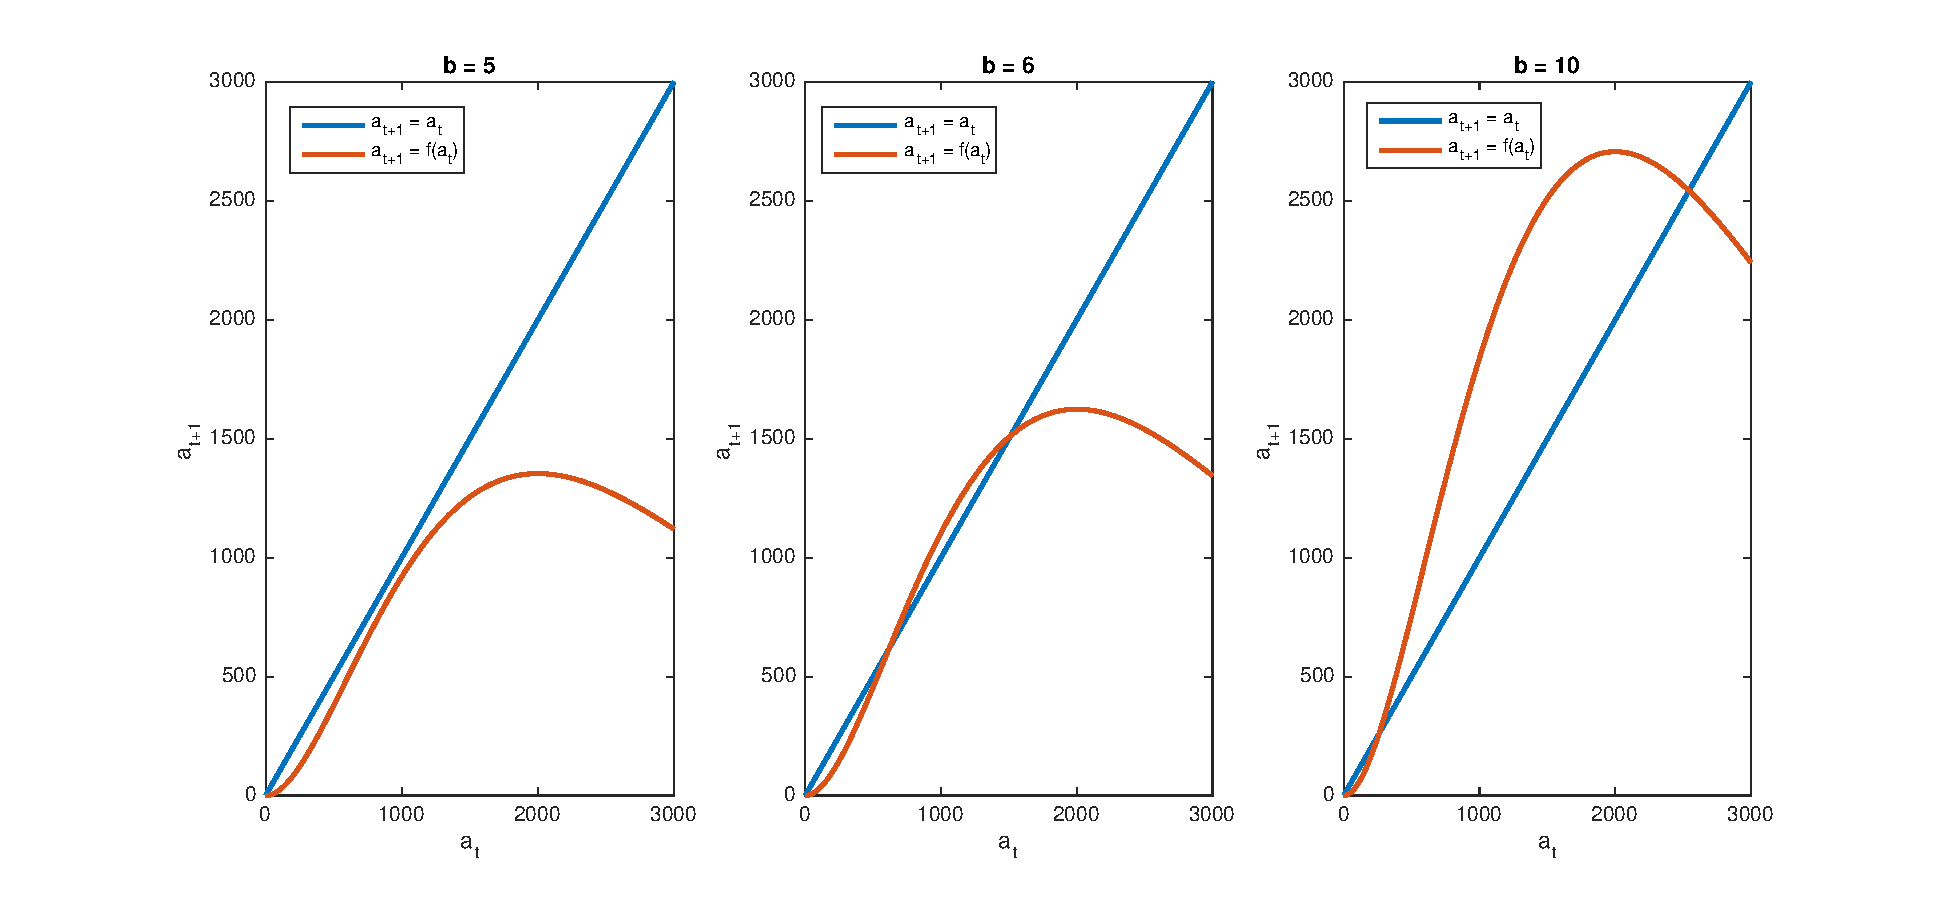
\includegraphics[scale=0.5]{figures/meanfield.eps}
	\caption{$a_{t+1}$ plotted against $a_t$. The blue lines are the $a_{t+1} = a_{t}$ whereas the red lines follow $a_{t+1} = \frac{a_t^2e^\frac{-a_t}{n}}{2n} b$. In these simulations n = 1000.}
    \label{fig:mf}
\end{figure}
As we increase b even more, we maintain three roots as seen in figure \ref{fig:mf2} we maintain three steady states. Note that we have not proven this but we expect the system to maintain this behavior. This can be proven by noting that $lim_{a_t -> \infty} = 0$ and that $f(2000) > 2000$ and $f(1) < 1$ if $ b > 6$. Thus we know that we must have at least two intersection (other than $a_t = 0$). Note that this is for n = 1000.
\begin{figure}[htbp]
	\centering
	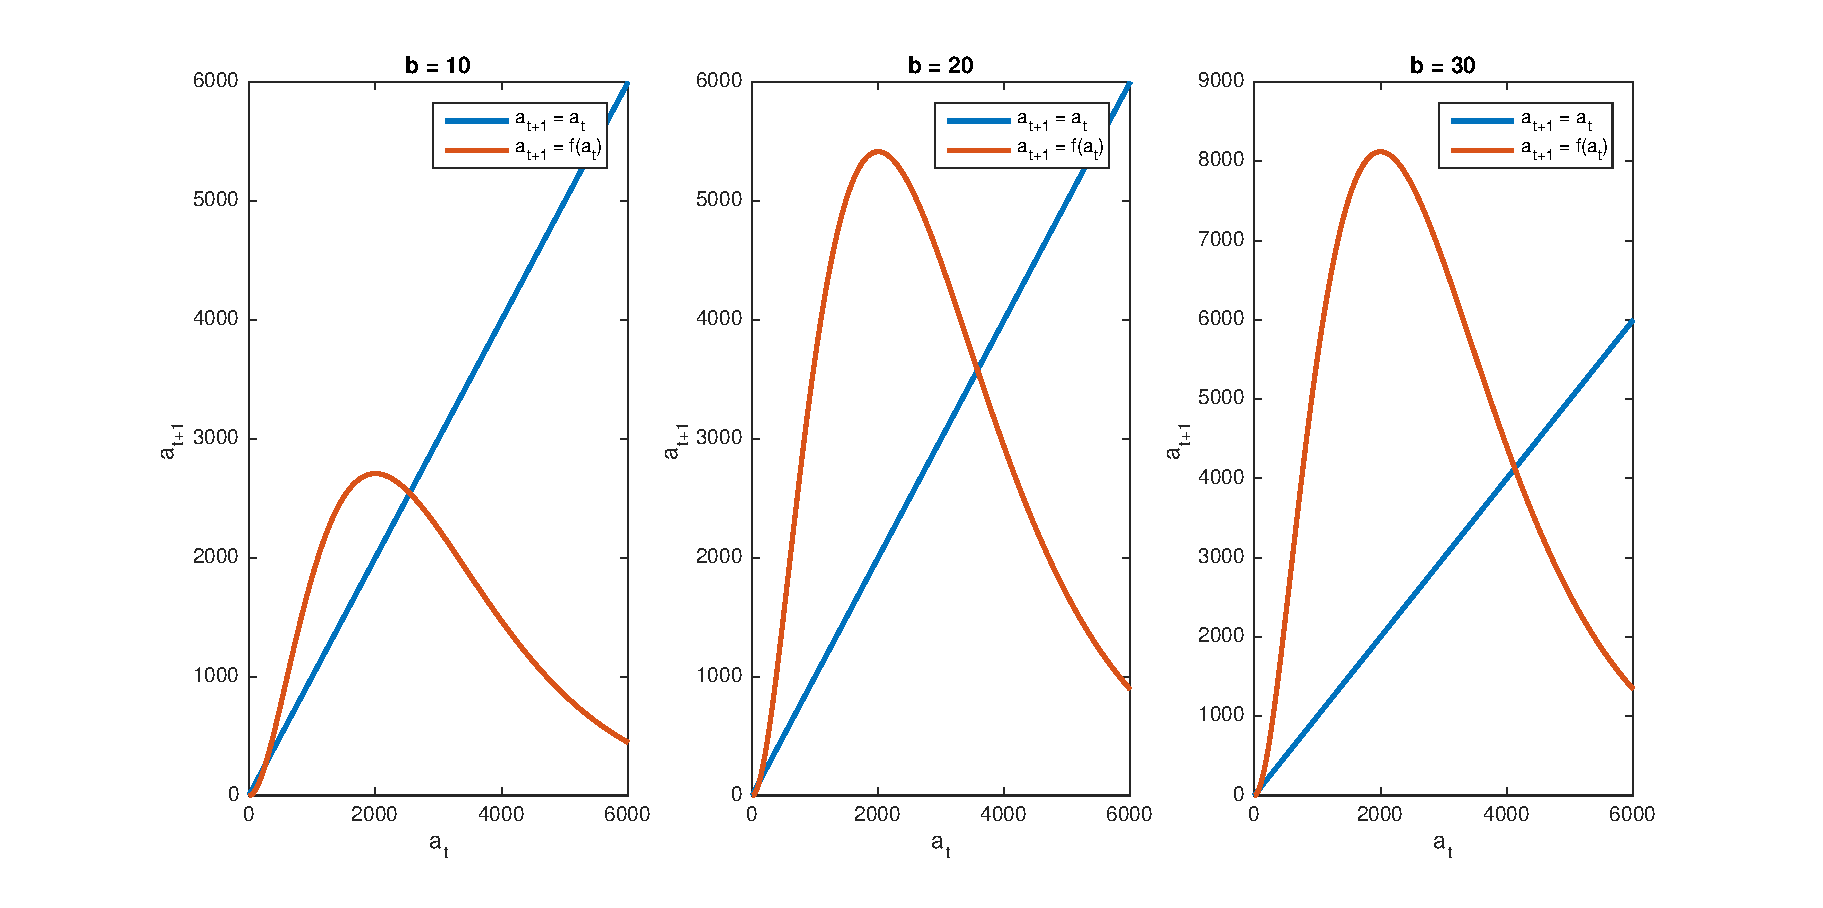
\includegraphics[scale=0.5]{figures/meanfield2.eps}
	\caption{$a_{t+1}$ plotted against $a_t$. The blue lines are the $a_{t+1} = a_{t}$ whereas the red lines follow $a_{t+1} = \frac{a_t^2e^\frac{-a_t}{n}}{2n} b$. In these simulations n = 1000.}
    \label{fig:mf2}
\end{figure}
%should we prove that for >5 we have 

\newpage
.
\newpage
\begin{appendix}{Appendix code for part A}\\ \\
Main function
\begin{lstlisting}
\end{lstlisting}
\end{appendix}
\end{document}
              